\chapter{Tecnologías y recursos}
\label{chap:tecnologia}

\drop{E}{n} esta sección se presentarán y detallarán los recursos hardware, lenguajes de programación, librerías y programas utilizados a lo largo del desarrollo de \MineRVa.

\section{Recursos hardware}

Este proyecto necesita de periféricos especiales para trabajar con tecnologías \acs{VR}, por lo que los recursos hardware de este proyecto son más exigentes.

\begin{itemize}
 \item \textbf{Lenovo Explorer.} Heatset \acs{VR} que se utilizará a lo largo del desarrollo. Incluye dos controladores, que son los que el usuario utilizará como interfaz al mundo virutal.

 \item \textbf{Asus R510V.} Ordenador en el que se comenzó la práctica, y que por motimos técnicos hubo de cambiar a mitad del proyecto. Cuenta con un procesador Intel i7-6700HQ, una memoria RAM DDR4 de 8GB, un disco dur  HyberX Kingston SSD de 256GB y una tarjeta gráfica NVIDIA GeForce GTX 950M.
 
 \item \textbf{Lenovo Legion Y530.} Es el segundo ordenador con el que se trabajó y con el que se terminó el proyecto. Cuenta con un procesador Intel i5-8300H, una memoria RAM DDR4 de 8GB, un disco dur  HyberX Kingston SSD de 256GB y una tarjeta gráfica NVIDIA GeForce GTX 1050.
 
\end{itemize}

\section{Recursos software}

Al haber trabajado con distintas tecnologías, los recursos software de este proyecto son variados, y se presentan a continuación.

\subsection{Sistema Operativo}

Se ha elegido trabajar con \textbf{Windows 10}, ya que es el que proporciona mejor soporte para los entornos y librerías de desarrollo, además de ser el que se espera que tengan la mayoría de usuarios de \MineRVa. Concretamente, se ha utilizado la versión \textbf{Edutation}, ya que se cuenta con licencia de la misma por ser estudiantes.

\subsection{Principales librerías}

\begin{itemize}
    \item \textbf{SteamVR\footnote{\url{http://steamvr.com}}} Es la principal librería para la que desarrollará, ya que es tanto la que mejor soporte tiene como la que más usuarios se espera que tengan o que más fácil sea para ellos descargar, ya que se encarga de ello Steam automáticamente.
    
\begin{figure}[!h]
\begin{center}

\includegraphics[width=0.35\textwidth]{imagenes/4/steamvr-logo.jpg}
\caption{Logo de SteamVR}
\label{fig:steamvr-logo}
\end{center}
\end{figure}

    \item \textbf{Windows Mixed Reality for SteamVR\footnote{\url{https://store.steampowered.com/app/719950/}}.} Es el wrapper necesario para utilizar el SDK de Steam con las gafas elegidas, ya que utilizan Windows Mixed Reality funcionar, que es una plataforma desarrollada por Microsoft para trabajar con \acs{MR}. Del mismo modo que SteamVR, se descarga automáticamente a través de Steam.

\begin{figure}[!h]
\begin{center}
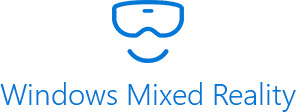
\includegraphics[width=0.35\textwidth]{imagenes/4/wmr-logo.jpg}
\caption{Logo de Windows Mixed Reality}
\label{fig:wmr-logo}
\end{center}
\end{figure}

    \item \textbf{VRTK\footnote{\url{https://vrtoolkit.readme.io/}}\footnote{\url{https://vrtoolkit.readme.io}}.} Es un framework de desarrollo multi-librería desarrollado en solitario por \textit{TheStoneFox} que permite desarrollar y compilar paralelamente para distintas librerías a través de una interfaz común, lo que le ha convertido en uno de los más utilizado del mercado.
    
\begin{figure}[!h]
\begin{center}

\includegraphics[width=0.35\textwidth]{imagenes/4/vrtk-logo.jpg}
\caption{Logo de VRTK}
\label{fig:vrtk-logo}
\end{center}
\end{figure}

\end{itemize}

\subsection{Herramientas de desarrollo}

\begin{itemize}
    \item \textbf{Unity\footnote{\url{https://unity.com/es}}.} (v2019.1.2) Es el \acs{IDE} elegido para desarrollar este proyecto. El lenguaje de desarrollo para trabajar con él es \texttt{C\#}, un lenguaje de programación orientado a objetos desarrollado y estandarizado por Microsoft  en el año 2000 que forma parte de su plataforma .NET.
    
    \item \textbf{Blender\footnote{\url{https://blender.org}}.} (v2.79b) es un programa informático multi plataforma, dedicado especialmente al modelado, iluminación, animación y renderizado de gráficos tridimensionales que se utilizará para modelar las salas del museo.
    
    \item \textbf{Visual Studio Community\footnote{\url{https://visualstudio.com/vs/community/}}.} (v2019) Es un \acs{IDE} desarrollado por Microsoft disponible para los principales sistemas operativos y que soporta una gran variedad de lenguajes. Es el editor por defecto que recomienda Unity, además de sincronizarse con él en tiempo real, por lo que será el utilizado para programar en C\#.
    
    \item \textbf{Atom\footnote{\url{https://atom.io}}.} Desarrollado por GitHub, es un \acs{IDE} de código abierto con soporte para extensiones desarrolladas por la comunidad e integración nativa con git, lo que lo hace especialmente potente para trabajar en todo tipo de proyectos. Se utilizará este programa para editar el resto de los archivos.
    
    \item \textbf{Git\footnote{\url{https://git-scm.com/}}.} Como herramienta de control de versiones se ha utilizado git, diseñado inicialmente por Linus Torvalds, el padre de Linux. Además, los repositorios tanto del proyecto como de esta documentación estarán alojados en \textbf{GitHub} y pueden encontrarse respectivamente en los siguientes enlaces.
    
    \begin{center}
        \url{https://github.com/gomezportillo/mineRVa}
        \url{https://github.com/gomezportillo/mineRVa-doc}
    \end{center}
    
\end{itemize}

\subsection{Herramientas de documentación}

\begin{itemize}
    \item \textbf{\LaTeX.} Sistema de composición de texto que se ha utilizado para la edición de la documentación de este \acs{TFM} en PDF.
    
    \item \textbf{LibreOffice Writer.} (v5.5) Editor de documentos \textit{open source} que forma parte del paquete LibreOffice y que se ha utilizado para generar el resto de documentos, como la guía de salas o el \acs{GDD}. 
    
    \item \textbf{LibreOffice Draw.} (v5.5) Editor utilizado para generar diagramas y gráficos que también forma parte del paquete LibreOffice.
    
    \item \textbf{LibreOffice Calc.} (v5.5) Editor de hojas de cálculo utilizado para generar gráficas a partir de datos.
    
    \item \textbf{GIMP.} (v2.10.8) Editor de imágenes \textit{open source}, multiplataforma y muy potente, aunque solo puede trabajar con gráficos rasterizados. Sus siglas significan \textit{GNU Image Manipulation Program}.
    
    \item \textbf{Inkscape.} (v0.92) Editor de imágenes utilizado para trabajar con los gráficos vectoriales del proyecto.
\end{itemize}